% Options for packages loaded elsewhere
\PassOptionsToPackage{unicode}{hyperref}
\PassOptionsToPackage{hyphens}{url}
%
\documentclass[
]{article}
\usepackage{lmodern}
\usepackage{amssymb,amsmath}
\usepackage{ifxetex,ifluatex}
\ifnum 0\ifxetex 1\fi\ifluatex 1\fi=0 % if pdftex
  \usepackage[T1]{fontenc}
  \usepackage[utf8]{inputenc}
  \usepackage{textcomp} % provide euro and other symbols
\else % if luatex or xetex
  \usepackage{unicode-math}
  \defaultfontfeatures{Scale=MatchLowercase}
  \defaultfontfeatures[\rmfamily]{Ligatures=TeX,Scale=1}
\fi
% Use upquote if available, for straight quotes in verbatim environments
\IfFileExists{upquote.sty}{\usepackage{upquote}}{}
\IfFileExists{microtype.sty}{% use microtype if available
  \usepackage[]{microtype}
  \UseMicrotypeSet[protrusion]{basicmath} % disable protrusion for tt fonts
}{}
\makeatletter
\@ifundefined{KOMAClassName}{% if non-KOMA class
  \IfFileExists{parskip.sty}{%
    \usepackage{parskip}
  }{% else
    \setlength{\parindent}{0pt}
    \setlength{\parskip}{6pt plus 2pt minus 1pt}}
}{% if KOMA class
  \KOMAoptions{parskip=half}}
\makeatother
\usepackage{xcolor}
\IfFileExists{xurl.sty}{\usepackage{xurl}}{} % add URL line breaks if available
\IfFileExists{bookmark.sty}{\usepackage{bookmark}}{\usepackage{hyperref}}
\hypersetup{
  pdftitle={Factor 2019-2020 Final Report},
  pdfcreator={LaTeX via pandoc}}
\urlstyle{same} % disable monospaced font for URLs
\usepackage{color}
\usepackage{fancyvrb}
\newcommand{\VerbBar}{|}
\newcommand{\VERB}{\Verb[commandchars=\\\{\}]}
\DefineVerbatimEnvironment{Highlighting}{Verbatim}{commandchars=\\\{\}}
% Add ',fontsize=\small' for more characters per line
\newenvironment{Shaded}{}{}
\newcommand{\AlertTok}[1]{\textcolor[rgb]{1.00,0.00,0.00}{\textbf{#1}}}
\newcommand{\AnnotationTok}[1]{\textcolor[rgb]{0.38,0.63,0.69}{\textbf{\textit{#1}}}}
\newcommand{\AttributeTok}[1]{\textcolor[rgb]{0.49,0.56,0.16}{#1}}
\newcommand{\BaseNTok}[1]{\textcolor[rgb]{0.25,0.63,0.44}{#1}}
\newcommand{\BuiltInTok}[1]{#1}
\newcommand{\CharTok}[1]{\textcolor[rgb]{0.25,0.44,0.63}{#1}}
\newcommand{\CommentTok}[1]{\textcolor[rgb]{0.38,0.63,0.69}{\textit{#1}}}
\newcommand{\CommentVarTok}[1]{\textcolor[rgb]{0.38,0.63,0.69}{\textbf{\textit{#1}}}}
\newcommand{\ConstantTok}[1]{\textcolor[rgb]{0.53,0.00,0.00}{#1}}
\newcommand{\ControlFlowTok}[1]{\textcolor[rgb]{0.00,0.44,0.13}{\textbf{#1}}}
\newcommand{\DataTypeTok}[1]{\textcolor[rgb]{0.56,0.13,0.00}{#1}}
\newcommand{\DecValTok}[1]{\textcolor[rgb]{0.25,0.63,0.44}{#1}}
\newcommand{\DocumentationTok}[1]{\textcolor[rgb]{0.73,0.13,0.13}{\textit{#1}}}
\newcommand{\ErrorTok}[1]{\textcolor[rgb]{1.00,0.00,0.00}{\textbf{#1}}}
\newcommand{\ExtensionTok}[1]{#1}
\newcommand{\FloatTok}[1]{\textcolor[rgb]{0.25,0.63,0.44}{#1}}
\newcommand{\FunctionTok}[1]{\textcolor[rgb]{0.02,0.16,0.49}{#1}}
\newcommand{\ImportTok}[1]{#1}
\newcommand{\InformationTok}[1]{\textcolor[rgb]{0.38,0.63,0.69}{\textbf{\textit{#1}}}}
\newcommand{\KeywordTok}[1]{\textcolor[rgb]{0.00,0.44,0.13}{\textbf{#1}}}
\newcommand{\NormalTok}[1]{#1}
\newcommand{\OperatorTok}[1]{\textcolor[rgb]{0.40,0.40,0.40}{#1}}
\newcommand{\OtherTok}[1]{\textcolor[rgb]{0.00,0.44,0.13}{#1}}
\newcommand{\PreprocessorTok}[1]{\textcolor[rgb]{0.74,0.48,0.00}{#1}}
\newcommand{\RegionMarkerTok}[1]{#1}
\newcommand{\SpecialCharTok}[1]{\textcolor[rgb]{0.25,0.44,0.63}{#1}}
\newcommand{\SpecialStringTok}[1]{\textcolor[rgb]{0.73,0.40,0.53}{#1}}
\newcommand{\StringTok}[1]{\textcolor[rgb]{0.25,0.44,0.63}{#1}}
\newcommand{\VariableTok}[1]{\textcolor[rgb]{0.10,0.09,0.49}{#1}}
\newcommand{\VerbatimStringTok}[1]{\textcolor[rgb]{0.25,0.44,0.63}{#1}}
\newcommand{\WarningTok}[1]{\textcolor[rgb]{0.38,0.63,0.69}{\textbf{\textit{#1}}}}
\usepackage{longtable,booktabs}
% Correct order of tables after \paragraph or \subparagraph
\usepackage{etoolbox}
\makeatletter
\patchcmd\longtable{\par}{\if@noskipsec\mbox{}\fi\par}{}{}
\makeatother
% Allow footnotes in longtable head/foot
\IfFileExists{footnotehyper.sty}{\usepackage{footnotehyper}}{\usepackage{footnote}}
\makesavenoteenv{longtable}
\usepackage{graphicx}
\makeatletter
\def\maxwidth{\ifdim\Gin@nat@width>\linewidth\linewidth\else\Gin@nat@width\fi}
\def\maxheight{\ifdim\Gin@nat@height>\textheight\textheight\else\Gin@nat@height\fi}
\makeatother
% Scale images if necessary, so that they will not overflow the page
% margins by default, and it is still possible to overwrite the defaults
% using explicit options in \includegraphics[width, height, ...]{}
\setkeys{Gin}{width=\maxwidth,height=\maxheight,keepaspectratio}
% Set default figure placement to htbp
\makeatletter
\def\fps@figure{htbp}
\makeatother
\setlength{\emergencystretch}{3em} % prevent overfull lines
\providecommand{\tightlist}{%
  \setlength{\itemsep}{0pt}\setlength{\parskip}{0pt}}
% \setcounter{secnumdepth}{-\maxdimen} % remove section numbering

\title{Factor 2019-2020 Final Report}
\author{Max Denning, Cameron Krimsky, \\ Cole Kurashige, Nandeeka Nayak, Kye Shi}
\date{May 8th, 2020}

\begin{document}
\maketitle

% \hypertarget{about-this-project}{%
% \section{About This Project}\label{about-this-project}}

\begin{abstract}
The goal of this project is to make non-trivial improvements to Factor.
There are many avenues for a concerted effort to grow Factor in an
organized and consistent manner. Any programming language can benefit
from this sort of effort, Factor included. After consulting with the
Factor maintainer \href{https://re-factor.blogspot.com/}{John}, we
narrowed down this open-ended goal to two projects: creating an online
platform for learning and using Factor and implementing a numerical
programming vocabulary in Factor.

This document provides summaries and methods for each project, as well as
possible areas for further development.
\end{abstract}

\hypertarget{the-factor-online-platform}{%
\section{The Factor Online Platform}\label{the-factor-online-platform}}

Factor is a great programming language, but has yet to break into the
mainstream. We think that easing the learning process will help to
improve its rate of adoption. Our online platform targets three aspects
that could make the language more inviting to new programmers: lowering
the installation barrier, adding more tutorials and learning materials,
and creating a documentation search engine.

\hypertarget{the-online-factor-interpreter}{%
\subsection{The online Factor
interpreter}\label{the-online-factor-interpreter}}

Suppose you're a newcomer to Factor (maybe you are), looking to try out
Factor because you read on some blog post about the interesting
language/syntax features that Factor has, or simply because you wanted
to get a feel for what it was like to write Factor code.

In order to do that, you would first have to download and install Factor
on your computer---either from Factor's website, or by cloning Factor's
GitHub repository and compiling Factor from source. To be sure, doing so
is not \emph{difficult}---but for many users who are merely looking to
experiment with Factor, having to go through the entire download/install
process is enough to discourage them from trying Factor.

The solution, inspired by existing tools for many other popular
languages (e.g., the Go Playground, Repl.it, JSFiddle, Try Haskell) and
various online coding course platforms (e.g., Codeacademy, Khan Academy,
freeCodeCamp), is a \href{https://factor.netlify.com}{\emph{web-based
interpreter} for Factor}. A web-based Factor interpreter removes the
aforementioned accessibility barrier: to get started with Factor, a user
does not need to download or install anything---only navigate to the
Factor interpreter website (at
\href{https://factor.netlify.com}{factor.netlify.com})---and they can
start exploring right away.

\hypertarget{goals-and-design-decisions}{%
\subsubsection{Goals and design
decisions}\label{goals-and-design-decisions}}

Factor, in its current form, is a self-hosted, compiled language. In
other words, its compiler is written in Factor as well. This form
doesn't lend itself well to being ported online for two reasons: -
first, the compiler outputs machine code (e.g., x86) meant for physical
CPUs, not Javascript (or even WebAssembly), the language needed for web
applications; - second, in order to port the Factor compiler to
Javascript, we would first have to port Factor to Javascript, since
Factor's compiler is written in Factor. These two reasons meant that we
couldn't get away with something as simple as ``use a X-to-Javascript
transpiler that someone else wrote'' to translate the Factor interpreter
to Javascript; instead, we would have to understand the mechanics of
Factor and write our own Factor interpreter---from scratch---in a
web-friendly language (Javascript, or something that compiles to
Javascript).

Given that requirement, we recognized it would not be realistic to fully
replicate the behavior of Factor within our one-school-year timeline.
Thus, keeping in mind that the intent of this project was to make Factor
more beginner-friendly, we prioritized the following goals: - implement
a core subset of Factor functionality, enough to demonstrate what
``Factor is like''; - provide features that make it easy and fun to
learn Factor (e.g., helpful error messages, interactivity); - supplement
the interpreter with tutorials and documentation-searching tools (more
in the Tutorials and Foogle sections), à la online coding course
platforms. Furthermore, we decided to implement the interpreter in
\href{https://elm-lang.org/}{Elm}, a functional programming language for
web applications known for its type safety (virtually no runtime
errors!), performance, and work in user-friendly compilers and error
messages.

\hypertarget{the-implementation}{%
\subsubsection{The implementation}\label{the-implementation}}

As we mentioned in the previous section, our online Factor interpreter
is written in Elm. This section will discuss, at a high level, the
architecture and the parts that fit together to make it work. To get
into the finer details, you can find our source code
\href{https://github.com/factor-hmc/simple-interpreter}{on GitHub}.

\hypertarget{the-elm-architecture}{%
\paragraph{The Elm architecture}\label{the-elm-architecture}}

If you're not familiar with the Elm architecture, it may be a good idea
to \href{https://guide.elm-lang.org/architecture/}{read about that}
first (it's the same ``architecture'' that inspired the design of
React/Redux, Vue/Vuex, and many other modern Javascript web frameworks).
The gist of the Elm architecture is this: the entire application state
(or ``model''; this is stuff like the contents of every text field, the
data to be displayed, the currently focused tab, etc.) is stored
globally. Every time an event happens (e.g., a button is clicked, the
contents of a text field changes, an API call returns a result), a
``message'' is emitted, and the model is updated using an
\texttt{update} function. This takes in a message and the current model
and returns the \emph{next} model, or how the model should look after
the message/event occurs. Each time the model is updated, a
\texttt{view} function is used to render the model to HTML.

\hypertarget{the-parts}{%
\paragraph{The parts}\label{the-parts}}

The online interpreter platform comprises several sub-applications: one
for the actual interpreter interface (\texttt{Terminal.elm}), one for
loading tutorials (\texttt{Book.elm}), and one for interfacing with the
Foogle API (\texttt{Foogle.elm}). Each sub-application lives in its own
Elm-architecture-like loop, with its own model, messages, and
\texttt{update} and \texttt{view} functions. Occasionally, in order to
have different sub-applications interact with each other (e.g., clicking
on the \texttt{➦} arrow in a code block copies the code from the
tutorials app and pastes it in the interpreter app), messages from one
sub-application are passed to another sub-application; in this way, the
various sub-applications are tied together by the main, root-level
application module (\texttt{App.elm}).

In addition to the sub-applications, a separate collection of modules
(prefixed \texttt{Factor.*}) handle the definitions (\texttt{Lang.elm}),
parsing (\texttt{Parser.elm}), evaluation (\texttt{Runtime.elm}), and
rendering (\texttt{Show.elm}) of Factor code and are used by the
interpreter interface to actually run Factor code. Since the Factor
modules don't, strictly speaking, constitute an ``app'', they aren't
subjected to the model-view-message-update Elm architecture. However,
they are organized similarly: - \texttt{Lang.elm} contains data type
definitions amounting to Factor objects and syntax trees; -
\texttt{Runtime.elm} defines a Factor runtime model (type
\texttt{State}, which stores information such as the current stack
contents and a word definition lookup table) and implements how
evaluating a piece of Factor code ``updates'' the state (function
\texttt{evalWords}); - \texttt{Show.elm} defines how different Factor
values (numbers, strings, quotations) are rendered to text/HTML output.

\hypertarget{future-work-contributing}{%
\subsubsection{Future work \&
contributing}\label{future-work-contributing}}

Below are a few areas in which the online Factor interpreter/platform
needs the most improvement, before the online interpreter can be truly
usable \& useful for the general Factor community.

\hypertarget{compatibility-with-existing-factor-mechanics}{%
\paragraph{Compatibility with existing Factor
mechanics}\label{compatibility-with-existing-factor-mechanics}}

Currently, the web-based Factor interpreter is largely an
\emph{approximation} of how Factor actually works: the subset of Factor
that is supported in the web-interpreter is fairly narrow, and even
among that subset, behavior on the web-interpreter differs (sometimes in
subtle ways) from Factor's current behavior. Here are a few examples:

\begin{itemize}
\item
  \textbf{Tokenizing and parsing.} In many other languages, syntax for
  special constructs like function definitions and array literals are
  hard-coded into the language's grammar and parser. On the other hand,
  Factor uses
  \href{https://docs.factorcode.org/content/article-parsing-words.html}{parsing
  words} to handle most of its special syntax: word (function)
  definitions are processed by the parsing words
  \href{https://docs.factorcode.org/content/word-__colon__,syntax.html}{\texttt{:}}
  and terminated by
  \href{https://docs.factorcode.org/content/word-\%3B\%2Csyntax.html}{\texttt{;}},
  array literals by
  \href{https://docs.factorcode.org/content/word-\%7B,syntax.html}{\texttt{\{}},
  and so on. A key benefit of this approach is that it allows endless
  customization of Factor's syntax and the construction of various
  domain-specific languages (DSLs) in native Factor code. To name a few
  examples:

  \begin{itemize}
  \tightlist
  \item
    \href{https://docs.factorcode.org/content/vocab-pair-rocket.html}{\texttt{pair-rocket}}
    defines
    \href{https://docs.factorcode.org/content/word-\%3D__gt__\%2Cpair-rocket.html}{\texttt{=\textgreater{}}},
    an alternative way to denote pairs in an ``associative'' container
    (e.g., a dictionary);
  \item
    \href{https://docs.factorcode.org/content/article-peg.ebnf.html}{EBNF}
    parsing words define a DSL that automatically synthesizes
    \href{https://en.wikipedia.org/wiki/Parsing_expression_grammar}{PEG-parsers}
    from grammars expressed in
    \href{https://en.wikipedia.org/wiki/Extended_Backus\%E2\%80\%93Naur_form}{EBNF}
    syntax, reminiscent of parser-generator solutions such as
    \texttt{lex} and \texttt{yacc} for other languages;
  \item
    \href{https://docs.factorcode.org/content/article-syntax-hashtables.html}{Hash
    tables},
    \href{https://docs.factorcode.org/content/article-hash-sets.html}{hash
    sets},
    \href{https://docs.factorcode.org/content/article-trees.html}{binary
    search trees}, and in fact \emph{arbitrary} containers/data
    structures may be constructed via custom-defined literal syntax
    words,
    e.g.~\href{https://docs.factorcode.org/content/word-H\%7B,syntax.html}{\texttt{H\{}},
    \href{https://docs.factorcode.org/content/word-HS\%7B,syntax.html}{\texttt{HS\{}},
    \href{https://docs.factorcode.org/content/word-TREE\%7B,trees.html}{\texttt{TREE\{}},
    etc.
  \end{itemize}

  This limitless customization of Factor's syntax and parsing behavior
  is part of what makes Factor a uniquely flexible programming language.
  So while working with parsing words aren't essential to a beginner's
  understanding \emph{of} Factor, they arguably \emph{are} essential to
  an authentic experience of what it is like to work with Factor.

  Currently, the web-based interpreter does not use parsing words.
  Instead, it takes the conventional approach and hard-codes a few
  special syntax words (\texttt{\{} for array literals, \texttt{{[}} for
  quotation literals, \texttt{:} for word definitions, etc.) to deal
  with the most common use cases; a more authentic approach would be to
  replicate Factor's actual parser behavior, which may be summarized as
  follows:

  \begin{itemize}
  \item
    Every Factor word is either an \emph{ordinary word} or a
    \emph{parsing word}. Ordinary words (e.g., \texttt{+},
    \texttt{print}) are essentially non-syntax, callable, ``function''
    words. Parsing words (e.g.~\texttt{V\{}, \texttt{::}, \texttt{\{},
    \texttt{{[}}, \texttt{=\textgreater{}}), on the other hand, define
    custom parsing behavior, such as special constructs, container
    literals and DSLs.
  \item
    During parsing, Factor keeps an \emph{accumulator vector}, which
    stores a list of ``instructions'' (e.g., push the number \texttt{13}
    onto the stack; push a quotation on the stack; call the word
    \texttt{times} on the current stack contents). The accumulator
    vector amounts to a mutable ``syntax tree'' for Factor code during
    parsing.

    Given a piece of Factor code, the parser first splits the code into
    tokens by whitespace (the ``tokenize'' step), then processes each
    token in order. For each token:

    \begin{itemize}
    \tightlist
    \item
      If the token is a literal string or number, a corresponding
      ``push'' instruction is added to the accumulator vector. For
      instance, \texttt{12} adds a ``push the number \texttt{12} onto
      the stack'' instruction to the accumulator.
    \item
      if the token is an ordinary word, a corresponding ``call''
      instruction is added to the accumulator vector. For instance,
      \texttt{+} adds a ``call the function \texttt{+} on the current
      stack contents'' instruction to the end of the accumulator.
    \item
      \emph{If the token is a parsing word}, it is \emph{not} added to
      the accumulator vector---instead, it is executed immediately,
      running special parsing primitives to parse code occurring after
      it and modifying the accumulator vector accordingly. For instance,
      \texttt{\{} interrupts normal Factor parsing, consumes tokens
      until a \texttt{\}} is found, creates an array with elements
      initialized from the items it parses, and adds a ``push this array
      onto the stack'' instruction to the accumulator.
    \end{itemize}
  \end{itemize}

  You can read more about Factor's parsing mechanics and how parsing
  words work
  \href{https://docs.factorcode.org/content/article-parsing-words.html}{in
  the official Factor documentation}.
\item
  \textbf{Name resolution and recursion}. Currently, words are stored
  internally as lists of instructions (push, call, etc.). A lookup table
  is used during evaluation to map word names to the corresponding
  instructions. When a new word is defined in terms of existing words,
  we construct the instruction list for the new word by
  \emph{concatenating} the instruction lists of words used in the
  definition. For example, if we define

\begin{verbatim}
: addmul ( a b c -- d ) + * ;
\end{verbatim}

  then the instruction list for \texttt{addmul} is constructed by
  concatenating the instruction list for \texttt{+} (obtained via the
  lookup table) with the instruction list for \texttt{*}.

  There are a few drawbacks to this approach, or at least the current
  implementation:

  \begin{itemize}
  \item
    \emph{It's inefficient.} Concatenating lists takes O(n) time (w.r.t.
    the length of the first list---Elm's \texttt{List} type is
    implemented internally as a singly-linked list, as in many
    functional languages of the same genre, e.g., Haskell and OCaml) and
    \emph{doubles} the memory used to store the definitions.

    To illustrate the inefficiency, suppose a word \texttt{w} has
    instruction list {[}i1, i2, \ldots, in{]}, and we define another
    word \texttt{x} as \texttt{w\ drop} (whose instruction list contains
    a single built-in \texttt{drop} instruction, since \texttt{drop} is
    a primitive); then \texttt{x} will instruction list {[}i1, i2,
    \ldots, in, drop{]}. Note that instructions \texttt{i1,\ ...,\ in}
    are stored \emph{twice}, once in \texttt{w}, and once in \texttt{x}.

    The \emph{sensible} approach is to instead keep a ``reference'' to
    words used in the definition and call those references, rather than
    ``copying'' and concatenating the definitions. A previous attempt at
    implementing this approach involved simply storing the names, as
    strings, of words, and looking up those names when the word is
    called, but that leads to erratic behavior, as in the following
    example:

    \begin{enumerate}
    \def\labelenumi{\arabic{enumi}.}
    \tightlist
    \item
      \texttt{w} is defined;
    \item
      \texttt{x} is defined in terms of \texttt{w};
    \item
      \texttt{w} is redefined;
    \item
      when \texttt{x} is called, it \emph{should} use the original/old
      version of \texttt{w}, but because resolution happens at
      call-time, \texttt{x} now uses the new version of \texttt{w}.
    \end{enumerate}

    Concatenating instruction lists was a quick hack to avoiding the
    above behavior, but it is far from a good solution. It should be
    noted, also, that the current implementation does not do this
    copy/concatenation recursively: \emph{quotations} defined in terms
    of existing words are stored using the names of those words, rather
    than concatenations of their instruction lists; this means that if,
    in the above example, the definition \texttt{x} uses a
    \emph{quotation} containing \texttt{w}, and \texttt{w} is redefined,
    then when \texttt{x} is called still the new version is used. So our
    current solution is really, in some sense, the worst of both worlds.
  \item
    \emph{Recursion is impossible (sometimes).} It should be apparent
    that it is impossible to define a word directly in terms of itself
    (recursion from within a quotation is fine, since a quotation stores
    names rather than actual instruction lists), since if we were to try
    to define a word \texttt{w} in terms of itself, we would first try
    to find \texttt{w} in the table of existing words and concatenate
    \texttt{w} to itself---which would fail, since \texttt{w} is not yet
    defined! Or, if \texttt{w} were previously defined, redefining
    \texttt{w} in terms of ``itself'' doesn't actually recursively call
    itself; instead, wherever a ``recursive'' call to \texttt{w} is
    made, the \emph{previous} version of \texttt{w} is used instead.
  \end{itemize}

  A better way to handle word definitions is to combine lists ``by
  reference''. One way to do so while allowing self-referencing
  (recursive) definitions is described below:

  \begin{itemize}
  \item
    Define an \texttt{Instruction} type to be either a \texttt{Push} or
    \texttt{Call} variant: a \texttt{Push} variant denotes ``push some
    item onto the stack'', a \texttt{Call} variant denotes ``call this
    word/instruction list on the stack''.

    \begin{itemize}
    \item
      The \texttt{Push} variant should hold a single parameter of type
      \texttt{Literal}, the object to push onto the stack;
    \item
      The \texttt{Call} variant would hold a single parameter of type
      \texttt{List\ \ \ Instruction}, the instruction list to call on
      the stack.

      However, in this setup Elm's recursion system would prevent us
      from being able to define a self-referencing word such as
      \texttt{:\ a\ (\ -\/-\ )\ 1\ a\ ;} (yes, that example is one that
      has no practical use, but should still be theoretically possible
      to define), since traditional ``tying the knot'' methods for
      mutual/self-recursion are disallowed in Elm (read more about the
      problem \href{https://elm-lang.org/0.19.1/bad-recursion}{here}).
      The gist of the problem is that since \texttt{a} is defined in
      terms of itself, its instruction list must contain a \texttt{Call}
      variant holding, well, the instruction list itself. Since Elm
      evaluates expressions strictly, a recursive definition like this
      would cause Elm to recur infinitely.

      The solution is to explicitly ``lazify'' the recursion: instead of
      parametrizing \texttt{Call} with a \texttt{List\ Instruction}, we
      parametrize it with \emph{a function} that lazily returns a
      \texttt{List\ Instruction} when called. This allows us to apply a
      tie-the-knot technique without sending the Elm evaluator into an
      infinite recursive loop.
    \end{itemize}

    The code below illustrates a simplified example of this idea in
    action:

\begin{Shaded}
\begin{Highlighting}[]
\KeywordTok{type} \DataTypeTok{Instruction} 
  \OperatorTok{=} \DataTypeTok{Push} \DataTypeTok{Int}
  \OperatorTok{|} \DataTypeTok{Call}\NormalTok{ (() }\OperatorTok{{-}\textgreater{}} \DataTypeTok{List} \DataTypeTok{Instruction}\NormalTok{)}

\FunctionTok{a}\NormalTok{ : }\DataTypeTok{List} \DataTypeTok{Instruction}
\FunctionTok{a} \OperatorTok{=} \KeywordTok{let} \FunctionTok{lazy}\NormalTok{ () }\OperatorTok{=}\NormalTok{ [ }\DataTypeTok{Push} \DecValTok{1}\OperatorTok{,} \DataTypeTok{Call} \FunctionTok{lazy}\NormalTok{ ] }\KeywordTok{in} \FunctionTok{lazy}\NormalTok{ ()}
\end{Highlighting}
\end{Shaded}

    compared to what the code \emph{would} look like if Elm supported
    recursive definitions with laziness by default. Note that this code
    \emph{would not} work in Elm:

\begin{Shaded}
\begin{Highlighting}[]
\KeywordTok{type} \DataTypeTok{Instruction}
  \OperatorTok{=} \DataTypeTok{Push} \DataTypeTok{Int}
  \OperatorTok{|} \DataTypeTok{Call}\NormalTok{ (}\DataTypeTok{List} \DataTypeTok{Instruction}\NormalTok{)}

\FunctionTok{a}\NormalTok{ : }\DataTypeTok{List} \DataTypeTok{Instruction}
\FunctionTok{a} \OperatorTok{=}\NormalTok{ [ }\DataTypeTok{Push} \DecValTok{1}\OperatorTok{,} \DataTypeTok{Call} \FunctionTok{a}\NormalTok{ ]}
\end{Highlighting}
\end{Shaded}
  \end{itemize}
\item
  \textbf{Word definitions.} Currently, word definitions on the web
  interpreter are evaluated at run time, i.e., when a definition
  instruction is executed. In Factor, word definitions are evaluated at
  parse time. To illustrate the difference, consider the following piece
  of code, wherein we define a word from within a quotation:

\begin{verbatim}
[ : add1 ( n -- m ) 1 + ; ]
5 add1
\end{verbatim}

  In desktop Factor, \texttt{:} is executed as soon as it is encountered
  (since it is a parsing word), parsing and loading the definition
  \texttt{add1} immediately. Thus an \emph{empty} quotation is pushed on
  to the stack (all tokens were consumed by the parsing process of
  \texttt{:}), \texttt{add1} is immediately defined and can be
  subsequently applied on \texttt{5}.

  On the current web interpreter, \texttt{:} is \emph{not} executed at
  parse time. Instead, it is parsed as a special ``definition''
  instruction and stored in the quotation as though it were a special
  word. Thus a quotation containing the ``definition'' instruction is
  pushed onto the stack, \texttt{add1} would not be defined, and the
  subsequent \texttt{5\ add1} call would fail because \texttt{add1} is
  not defined. One would have to \texttt{call} the quotation to actually
  define \texttt{add1}.

  Of course, it could be argued that this method allows for some
  interesting behavior as well, but it is confusing and certainly
  doesn't match the expected Factor behavior. So it should be changed.
  Presumably, fixing parsing (see the first bullet point) and adding
  parsing words would fix this issue as well.
\item
  \textbf{Stack effects.} The current stack effect parser is incomplete:
  it can't handle any ``nested'' effects
  (e.g.~\texttt{(\ quot:\ (\ a\ -\/-\ b\ )\ seq\ -\/-\ \ \ seq\textquotesingle{}\ )}
  and doesn't parse any special tokens (e.g.~\texttt{!} for mutability,
  \texttt{..} for row polymorphism). It only accounts for
  space-delimited tokens separated by a \texttt{-\/-}. Furthermore,
  currently nothing useful is done with the stack effect---at a minimum,
  there should be some form of stack-checking/stack-inference used to
  verify word definitions.
\item
  \textbf{Miscellaneous language features.} Various language features,
  such as classes, tuples, mixins, generics, etc. are not implemented.
  The absence of these features prevents a significant portion of
  existing Factor code from working in the web interpreter.
\end{itemize}

\hypertarget{loading-existing-factor-vocabularies}{%
\paragraph{Loading existing Factor
vocabularies}\label{loading-existing-factor-vocabularies}}

Once Factor mechanics are replicated sufficiently in the web interpreter
per the above points, we will be able to properly load existing Factor
vocabularies (e.g., \texttt{combinators}, \texttt{sequences},
\texttt{math}, etc.). (Currently, only \texttt{kernel} and most of
\texttt{math} are available in the web-interpreter, and they were ported
manually with several dirty hacks, namely by pasting Factor code
straight into Elm and deleting code that used unsupported features.) The
proposed method for doing so is as follows:

\begin{itemize}
\item
  Implement a parsing word \texttt{USE:}, which calls a primitive ``load
  vocabulary'' instruction from the Elm-based runtime.
\item
  When the ``load vocabulary'' instruction is called, make an HTTP
  request to the official Factor GitHub repository to fetch the
  corresponding \texttt{.factor} source file (not having to keep a
  separate copy/version of the Factor source repository makes the
  interpreter easier to maintain; since the interpreter is meant as an
  experimental scratchpad anyway, version consistency \& stability
  aren't that important anyway). Parse the source file and load it in
  the interpreter runtime.
\end{itemize}

\hypertarget{general-ui-and-learner-friendly-improvements}{%
\paragraph{General UI and learner-friendly
improvements}\label{general-ui-and-learner-friendly-improvements}}

\begin{itemize}
\item
  The desktop Factor listener is highly interactive and introspective:
  most values are clickable and, when clicked, bring up dialogs
  presenting the contents/other details about the items clicked. The web
  interpreter lacks this feature.
\item
  We set out to make the web interpreter a low-barrier means for Factor
  newcomers to experiment with and learn Factor; key to this experience
  is helpful error reporting with user-friendly, intuitive error
  messages (see https://elm-lang.org/news/the-syntax-cliff,
  https://elm-lang.org/news/compilers-as-assistants,
  https://elm-lang.org/news/compiler-errors-for-humans). Currently, the
  web interpreter has \emph{no} error reporting features.
\item
  Syntax highlighting would be cool to have.
\end{itemize}

\hypertarget{tutorials}{%
\subsection{Tutorials}\label{tutorials}}

When we began learning Factor, we started by following the
\href{https://docs.factorcode.org/content/article-first-program.html}{``Your
First Program''} tutorial within the Listener. This tutorial taught us
the basics of Factor however, after we completed it we weren't sure
where to go next. There are a handful of beginner level resources that
we found online. In fact, we cataloged many of these other resources an
\href{https://factor.netlify.app/book/Resources.md}{``Other Resources''}
section. We decided that creating more tutorials could only help entice
new factor programmers. We have a listing of all our tutorials in our
\href{https://factor.netlify.app/book/Table_of_Contents.md}{``Table of
Contents''}.

\hypertarget{tutorial-structure}{%
\subsubsection{Tutorial Structure}\label{tutorial-structure}}

We decided to structure our tutorials into two categories. The first
teaches basic ideas of Factor like how the Stack works or how to write
Words. They also include an example that showcases the given idea in
action. Our current set of tutorials that belong to this first set are
on the following topics: -
\href{https://factor.netlify.app/book/the-stack.md}{The Stack} -
\href{https://factor.netlify.app/book/words.md}{Words} -
\href{https://factor.netlify.app/book/vocabularies.md}{Vocabularies} -
\href{https://factor.netlify.app/book/quotations_combinators.md}{Quotation
and Combinators}

The second set combines these basic ideas and shows how one might
approach coding a more complicated program. We currently only have one
tutorial for this set called
\href{https://factor.netlify.app/book/Super_Hello_World.md}{``Super
Hello World''} which walks through how someone might write a function
which prints something a certain number of times based on an input. You
can see a short summary of each tutorial in the
\href{tutorials.md}{Tutorial Summaries} section of this report. We also
have a
\href{https://factor.netlify.app/book/Table_of_Contents.md}{``Table of
Contents''} section which gives a short description of each tutorial so
that users can easily find which tutorial might be most beneficial to
them. We also have an
\href{https://factor.netlify.app/book/Resources.md}{``Other Resources''}
section which has a small collection of resources we consulted and found
helpful when learning Factor.

Our tutorials are being held on our Factor Online Platform along with
our interpreter and Foogle. These two other aspects of the platform help
to make the tutorials more interactive. When reading through the
tutorials, one can type sample code directly into the interpreter to see
what exactly each new line of Factor code introduced in the tutorial
does. In addition, certain snippets of code allow the user to click on
it in order to have it copied into the interpreter. This way a user can
see how exactly the piece of code should be written, as well as quickly
see what a snippet of code does if they do not want to type it
themselves. We hope that the ease of running example code helps sidestep
some common beginner mistakes like missing spaces or semicolons with
little frustration.

While Foogle does not directly interact with the tutorials, it is a
great resource that can introduce new Factor programmers to the variety
of vocabularies and words that they have access too. Newer programmers
can use Foogle to look up words mentioned in the tutorials to learn
about them as well as similar words. Foogle will also help facilitate
the next step in learning Factor after finishing the tutorials. Factor
users that take the next step and attempt their own projects will be
able to search for desired words faster. The interpreter, tutorials, and
Foogle all are able to help ease programmers into Factor.

\hypertarget{tutorial-summaries}{%
\subsubsection{Tutorial Summaries}\label{tutorial-summaries}}

We have a quick summary of each of the current the tutorials below:

\hypertarget{the-stack}{%
\paragraph{\texorpdfstring{\href{https://factor.netlify.app/book/the-stack.md}{The
Stack}:}{The Stack:}}\label{the-stack}}

This tutorial explains the concept of the stack as well as how Factor
Programming revolves around it. We explain how one pushes and pops items
from the stack and how a function applied to the stack will work. We
also give the user a collection of simple words which allow users to
manipulate objects on the stack (dup, drop, swap \ldots{} etc).

\hypertarget{words}{%
\paragraph{\texorpdfstring{\href{https://factor.netlify.app/book/words.md}{Words}:}{Words:}}\label{words}}

In this section, we explain that Factor's version of functions are known
as words. We then go on to explain how to write and use words.
Specifically, we go into depth about how to specify the correct number
of inputs and outputs a word will have and how words manipulate inputs
to produce a desired output. We also walkthrough the process of writing
a word step by step.

\hypertarget{vocabularies}{%
\paragraph{\texorpdfstring{\href{https://factor.netlify.app/book/vocabularies.md}{Vocabularies}:}{Vocabularies:}}\label{vocabularies}}

Here, we explore vocabularies and how they are essentially Factor's
version of a library. This tutorial shows how to import entire
vocabularies or single words from vocabularies to use in projects.

\hypertarget{quotations-and-combinators}{%
\paragraph{\texorpdfstring{\href{https://factor.netlify.app/book/quotations_combinators.md}{Quotations
and
Combinators}:}{Quotations and Combinators:}}\label{quotations-and-combinators}}

This tutorial covers quotations and combinators. It shows users how to
push blocks of code to the stack, and how combinators can make use of
them as inputs. It then showcases quotations and combinators in action
with a walkthrough that shows the creation of a word which outputs a
certain term in the fibonacci sequence based on a given input. We
believe that this section should highlight quotations and combinators as
important tools when developing complex programs.

\hypertarget{super-hello-world}{%
\paragraph{\texorpdfstring{\href{https://factor.netlify.app/book/Super_Hello_World.md}{Super
Hello World}:}{Super Hello World:}}\label{super-hello-world}}

This tutorial is inspired by the Hello World tutorial that every
programming language seems to have. After learning how to write a
program that prints ``hello world'', we then learn how to write a more
complicated program which prints ``hello world'' a specific number of
times. This section explores the thought process a Factor programmer
might go through when writing code. This tutorial also acts as a review
of the previous sections.

\hypertarget{future-work}{%
\subsubsection{Future work}\label{future-work}}

There are several aspects of our collection of tutorials that we would
like to improve. The first is that we would like to create more
tutorials which expand on the basic ideas we have taught and write more
complicated programs like the Super Hello World tutorial. We think that
showcasing the creation of more complicated projects will not only show
new Factor programmers how to approach building a larger Factor program,
but show off what Factor is capable of. For example, a tutorial which
involves creating a simple vocabulary that contains several words or a
tutorial demonstrating how to write a small ``choose your own
adventure'' program that accepts inputs during runtime could be added.
There are even more advanced Factor topics for which it would be nice to
have tutorials, like how to write unit tests or how to set up a class.

The second addition we would make is to ensure that every line of code
presented in the tutorial can be run in the interpreter. As of right
now, most of the code in the tutorials can be run on the interpreter.
However, there are still some Factor features which are not implemented
in the interpreter, meaning that following the tutorials requires
installing Factor. One tutorial that suffers from this is the
vocabularies tutorial. The interpreter does not let a user run the
\texttt{USE:} word to import any vocabularies. In the Super Hello World
tutorial, we run into a similar problem when we try to create the word
\texttt{:\ Super\_HW\ (\ n\ -\/-\ )\ 1\ swap\ {[}a,b{]}\ {[}\ "Hello\ World"\ print\ .\ {]}\ each\ ;}
which requires the use of the word \texttt{{[}a,b{]}} from the
\texttt{math.ranges} vocabulary and a combinator \texttt{each} which is
from the sequences vocabulary. It would make the learning experience
much smoother if this issues were fixed and we could type every line
straight into the online interpreter.

Another thing we would like to incorporate into our tutorials is user
feedback. Our tutorials have yet to be tested on new Factor learners. We
believe that giving these tutorials to new Factor programmers and then
receiving their feedback will allow us to target areas of the tutorials
that are lacking. One way this could be carried out is to assemble a
group of both experienced programmers and newer programmers. We would
then split them into two groups with an even mixture of veteran and
novice programmers on each. Give one group the tutorials from the Factor
Online Platform and the other a list of tutorials found elsewhere
online. Allow both groups some time to experiment with the tutorials
(maybe an hour). Then give each group a short quiz that tests their
ability to program in Factor as well as a short survey about what they
liked and disliked about each tutorial. This will allow us to see how
effective our tutorials our compared to others. It will also help
identity problems with our tutorials. We can also incorporate other
aspects of other tutorials that users found helpful into our own. A
second way to get feedback would be to create a feedback form on the
Factor Online Platform where users could suggest improvements on the
tutorials and other aspects of the platform.

\hypertarget{foogle}{%
\subsection{Foogle}\label{foogle}}

Suppose you're writing a program in Factor and you have a list which you
need to get the 7th element of. You don't know how to do this in Factor,
but you suspect there is a function that you can use. Foogle can find
this function for you. You give it the query

\begin{verbatim}
( n:number seq:sequence -- elt )
\end{verbatim}

and it gives you back a bunch of functions, among them \texttt{nth}, the
function you're looking for.

Foogle works by taking information about the inputs and outputs of a
function. In this case, you've specified that your function's first
input (\texttt{n}) is a \texttt{number} and its second input
(\texttt{seq}) is a \texttt{sequence}. You don't know any specific
information about its output, so you give it a name (\texttt{elt}) but
don't specify what type it has to be. Names are still important, since
even if you don't have type information about an input or output, if you
have a sense of what its name might be, that will help Foogle find it.
Using this information, Foogle finds functions in Factor that you might
be looking for.

Try it at \url{https://factor.netlify.com/foogle}.

\hypertarget{background-and-motivation}{%
\subsubsection{Background and
motivation}\label{background-and-motivation}}

Have you ever implemented a function that you know must exist already?
You just couldn't find what library it was in and what that library
called it. This is unsurprising. Even common operations like getting the
first element of a list can have different names between programming
languages:
\href{https://docs.factorcode.org/content/word-first,sequences.html}{first}
in Factor,
\href{https://hackage.haskell.org/package/base-4.12.0.0/docs/Data-List.html\#v:head}{head}
in Haskell, or
\href{https://www.gnu.org/software/emacs/manual/html_node/eintr/car-_0026-cdr.html}{car}
in Lisp.

Foogle is inspired by \href{https://hoogle.haskell.org/}{Hoogle}, a
function search engine for Haskell. Hoogle allows users to query
functions based on the types of their inputs and outputs. You might ask
why this is relevant to Factor, seeing as it is not statically typed.
Although Factor doesn't require type annotations, parameters typically
have some amount of type information associated with them. This either
is documented in naming conventions, like \texttt{seq} for
\texttt{sequence}s or \texttt{?} for \texttt{boolean}s, or in the help
page for the function, like for
\href{https://docs.factorcode.org/content/word-+,math.html}{\texttt{+}}
or
\href{https://docs.factorcode.org/content/word-nth\%2Csequences.html}{\texttt{nth}}.
In general, there is some form of identifying information about the
inputs and outputs of a function.

\hypertarget{building-running-and-deploying-foogle}{%
\subsubsection{Building, running, and deploying
Foogle}\label{building-running-and-deploying-foogle}}

Foogle depends on the Haskell package manager
\href{https://docs.haskellstack.org/en/stable/README/}{stack}.

\hypertarget{building}{%
\paragraph{Building}\label{building}}

To build, simply
\href{https://docs.haskellstack.org/en/stable/install_and_upgrade/}{install
stack} and run

\begin{verbatim}
$ stack build
\end{verbatim}

in the root.

\hypertarget{running}{%
\paragraph{Running}\label{running}}

To run the server locally, set the port you want to host the server on
(like 8001) as the environment variable PORT. For example,
\texttt{\$\ export\ PORT=8001}. Then run

\begin{verbatim}
$ stack exec foogle-server
\end{verbatim}

in the root. This will run the server at \texttt{http://localhost:8001}
(or whatever port you set it). You may then query the server with
\texttt{curl} to send GET requests.

You may also run the command-line interface locally, which is typically
easier to test new features. After building (building builds both the
server and application), run

\begin{verbatim}
$ stack exec foogle-exe -- [args] stack-effect
\end{verbatim}

to query. To figure out what args the executable supports, run

\begin{verbatim}
$ stack exec foogle-exe -- -h
\end{verbatim}

or

\begin{verbatim}
$ stack exec foogle-exe -- --help
\end{verbatim}

If you want to run the interpreter and Foogle locally, follow the
instructions on running the interpreter locally and change the
\texttt{endpoint} variable in
\href{https://github.com/factor-hmc/simple-interpreter/blob/master/src/Foogle.elm}{\texttt{Foogle.elm}}
to point to the localhost location
(e.g.~\texttt{http://localhost:8001}). 


\hypertarget{deploying}{%
\paragraph{Deploying}\label{deploying}}

Supposing that
ownership of the Heroku app was transferred to you, it should be
sufficient to connect your Heroku account and
\href{https://devcenter.heroku.com/articles/git}{push to the Heroku app
via git}. This will deploy the Foogle server on Heroku. The online
platform points to the Heroku app when it queries Foogle, so you won't
need to make changes there unless you change the URL at which Foogle is
hosted.

If you do not have ownership of the Heroku app (and cannot obtain it),
then you want to make a new one. Create it using
\href{https://github.com/mfine/heroku-buildpack-stack}{this buildpack}
and make sure to configure the run file to build and run
\texttt{foogle-server}.
\href{https://hackernoon.com/for-all-the-world-to-see-deploying-haskell-with-heroku-7ea46f827ce}{This
tutorial} may be helpful in setting the app up. Then change the
\texttt{endpoint} variable in
\href{https://github.com/factor-hmc/simple-interpreter/blob/master/src/Foogle.elm}{\texttt{Foogle.elm}}
to point to the new Heroku app.

\hypertarget{implementation}{%
\subsubsection{Implementation}\label{implementation}}

There are three components to Foogle's implementation and a fourth
auxiliary interface. 1. Database generator 2. Search engine 3. Frontend
4. Command-line application

First, we generate a database containing input-output information for
all of the functions in Factor. This database is read by the search
engine. The frontend is used to send queries to the search engine, which
returns them in a format that the frontend then displays to the user.

\hypertarget{database-generator}{%
\paragraph{Database generator}\label{database-generator}}

You can find the database generator generator at
\href{https://github.com/factor-hmc/foogle/blob/master/make-database.factor}{foogle/make-database.factor}.

The database generator is a simple script written in Factor that
iterates over each function and creates a JSON object documenting it.
These objects are described below.

Because of the way that pandoc converts Markdown tables to \LaTeX,
the tables below have been instead rendered as bulleted lists. It might be
easier to view them
\href{https://factor.netlify.app/book/about/online-platform/foogle/implementation.md#function-objects}{online}.

\hypertarget{function-objects}{%
\subparagraph{Function objects}\label{function-objects}}

\begin{itemize}
  \item \textbf{Key}: ``name''
    \begin{itemize}
      \item \textbf{Value Type}: String
      \item \textbf{Value Description}: Name of the function.
    \end{itemize}
  \item \textbf{Key}: ``effect''
    \begin{itemize}
      \item \textbf{Value Type}:
        Object or Boolean
      \item \textbf{Value Description}: 
        If the function has a stack effect, an object representing it.
        Otherwise, the value \texttt{false}.
    \end{itemize}
  \item \textbf{Key}: ``url''
    \begin{itemize}
      \item \textbf{Value Type}:
        String
      \item \textbf{Value Description}: 
      URL to the function's help page on the Factor documentation.
    \end{itemize}
  \item \textbf{Key}: ``vocabulary''
    \begin{itemize}
      \item \textbf{Value Type}:
        String
      \item \textbf{Value Description}: 
      Name of the function's vocabulary (library).
    \end{itemize}
  \item \textbf{Key}: ``vocabulary\_url''
    \begin{itemize}
      \item \textbf{Value Type}:
        String
      \item \textbf{Value Description}: 
      URL to the vocabulary's help page on the Factor documentation.
    \end{itemize}
\end{itemize}

\hypertarget{stack-effect-objects}{%
\subparagraph{Stack effect objects}\label{stack-effect-objects}}

\begin{itemize}
  \item \textbf{Key}: ``in''
    \begin{itemize}
      \item \textbf{Value Type}:
        Array
      \item \textbf{Value Description}: 
      List of input stack effect variables.
    \end{itemize}
  \item \textbf{Key}: ``out''
    \begin{itemize}
      \item \textbf{Value Type}:
        Array
      \item \textbf{Value Description}: 
      List of output stack effect variables.
    \end{itemize}
  \item \textbf{Key}: ``in\_var''
    \begin{itemize}
      \item \textbf{Value Type}:
        String or Boolean
      \item \textbf{Value Description}: 
      If the function has an input row variable, its name. Otherwise, the
      value \texttt{false}.
    \end{itemize}
  \item \textbf{Key}: ``out\_var''
    \begin{itemize}
      \item \textbf{Value Type}:
        String or Boolean
      \item \textbf{Value Description}: 
      If the function has an output row variable, its name. Otherwise, the
      value \texttt{false}.
    \end{itemize}
  \item \textbf{Key}: ``terminated?''
    \begin{itemize}
      \item \textbf{Value Type}:
        Boolean
      \item \textbf{Value Description}: 
      Does the function terminate in an error? Factor functions that do this
      usually have their output stack effect declared as \texttt{*}. See
      \href{https://docs.factorcode.org/content/word-decode-error\%2Cio.encodings.html}{this
      function} for an example.
    \end{itemize}
  \item \textbf{Key}: ``effect\_descriptions''
    \begin{itemize}
      \item \textbf{Value Type}:
        Object
      \item \textbf{Value Description}: 
      An object that has keys equal to the names of the stack effect variables
      and values equal to their description on the function's help page. It
      may not have all stack effect variables in it (in fact, it may have
      none).
    \end{itemize}
\end{itemize}

\hypertarget{effect-variables}{%
\subparagraph{Effect variables}\label{effect-variables}}

There are three possibilities for an effect variable's value.

\begin{itemize}
  \item \textbf{Variable Type}: Stack Effect Variable
    \begin{itemize}
      \item \textbf{Value Type}:
        String
      \item \textbf{Value Description}: 
        A string describing the name of the variable.
    \end{itemize}
  \item \textbf{Variable Type}: Typed Stack Effect Variable
    \begin{itemize}
      \item \textbf{Value Type}:
        Array
      \item \textbf{Value Description}: 
        An array of two strings. The first is the name of the variable and the
        second is the type of the variable.
    \end{itemize}
  \item \textbf{Variable Type}: Quotation Stack Effect Variable
    \begin{itemize}
      \item \textbf{Value Type}:
        Array
      \item \textbf{Value Description}: 
        An array of a string and an object. The string is the name of the
        variable. The object is a stack effect object representing its stack
        effect.
    \end{itemize}
\end{itemize}

The generator creates a database of all functions that are in Factor
when it is loaded (those obtained from the function \texttt{all-words}).
This should be all of the functions in the official Factor ecosystem.

This database is an array of function objects. It is not too difficult
to parse the database, but be aware that many values are heterogeneous
(i.e.~they can have more than one possible type). ``in\_var'' for effect
objects, for example, may be strings or the boolean value
\texttt{false}.

\hypertarget{search-engine}{%
\paragraph{Search engine}\label{search-engine}}

\hypertarget{overview}{%
\subparagraph{Overview}\label{overview}}

The search engine is a webserver written in Haskell using
\href{https://www.servant.dev/}{Servant}. It first parses the database
information. When it receives a query, it first parses the query into a
stack effect, then searches functions to find those with stack effect
closest to the query.

Parsing the database is not difficult, and follows the specification of
the JSON values.

The query parsing closely mimicks Factor's own parser for stack effects.
Tokens, for example, must be space-separated. A general description of
the form of stack effects can be found
\href{https://docs.factorcode.org/content/article-effects.html}{at this
webpage}. There are a few differences for Foogle's parser. First, it is
more permissive in what types of dashes it accepts as a separator
between in variables and out variables (it will accept unicode em
dashes, as searching on a phone can generate those by accident). Second,
it allows users to search by types as if they were writing a stack
effect declaration for a
\href{https://docs.factorcode.org/content/word-TYPED__colon__,typed.html}{TYPED:
function}. This syntax is of the form \texttt{effVarName:\ type}. It
also allows users to specify \emph{multiple} types for a given variable
by separating the type with a bar \texttt{\textbar{}}. These are
presently treated as a disjunction (i.e.~only one of the types needs to
match). Finally, it does not properly figure out whether an effect has
the property \texttt{terminated?}. It's very likely that adding this
property just requires that you check if the last effect variable in the
output effect is called \texttt{*}, but this wasn't confirmed.

An example query showcasing most of the differing features of the parser
is shown below. Comments are rendered after \texttt{!}, but this isn't
valid syntax for the parser (although it could be extended to allow it).

\begin{verbatim}
( var1: boolean            ! declare types like in the TYPED: effect
  var2: string | sequence  ! declare disjunction types
  —                        ! em-dash instead of --
  *                        ! parsed as a normal stack effect, 
                           ! when it probably should change the 
                           ! terminated? property
)
\end{verbatim}

Foogle conducts its searching using the metric of edit distance from one
stack effect to another, where insertions and deletions are
disincentivized. Effect variables with matching types have the most
incentive to being matched. If the types cannot be matched, the engine
attempts to match the names of the variables.

\hypertarget{code-description}{%
\subparagraph{Code description}\label{code-description}}

You can find the server code at
\href{https://github.com/factor-hmc/foogle/tree/master/server}{foogle/server}.
A summary of each file is provided below.

\href{https://github.com/factor-hmc/foogle/blob/master/server/Main.hs}{foogle/server/Main.hs}
compiles to the server executable. It loads the database and passes it
to a function that makes and runs the server.

\href{https://github.com/factor-hmc/foogle/blob/master/server/Server.hs}{foogle/server/Server.hs}
is the actual server code. The type of the API (\texttt{QueryAPI})
specifies the inputs the server accepts and the outputs it returns. The
\texttt{server} function implements the logic that validates inputs,
calls a function to search the database, and returns an array of JSON
objects (\texttt{FoogleResult}s). It uses
\href{https://www.servant.dev/}{Servant}.

The main Foogle and searching logic is in
\href{https://github.com/factor-hmc/foogle/tree/master/src}{foogle/src}.

\href{https://github.com/factor-hmc/foogle/blob/master/src/Types.hs}{foogle/src/Types.hs}
contains the definitions of most types and their implemented type
classes used by the search engine. Relevant type classes include the
\texttt{Show} instances, which describe how to render the various data
types, and the \texttt{FromJSON} instances, which describe how to parse
the types from JSON. The JSON parsing uses
\href{https://hackage.haskell.org/package/aeson}{Aeson}.

\href{https://github.com/factor-hmc/foogle/blob/master/src/EditDistance.hs}{foogle/src/EditDistance.hs}
is a (mostly copied) implementation of a dynamic-programming based edit
distance algorithm.

\href{https://github.com/factor-hmc/foogle/blob/master/src/Parse.hs}{foogle/src/Parse.hs}
is a parser for stack effects. It supports some custom features that
Factor doesn't, like parsing multiple types for a stack effect variable
as well as using unicode dashes instead of \texttt{-\/-} to separate
inputs and outputs (this is to help people searching on devices that
make \texttt{-\/-} into these unicode dashes). It uses
\href{https://hackage.haskell.org/package/megaparsec}{megaparsec} for
parsing.

\href{https://github.com/factor-hmc/foogle/blob/master/src/Infer.hs}{foogle/src/Infer.hs}
is where the search engine guesses types for the stack effect variables.
This is done by inspecting their names and documentation.

\href{https://github.com/factor-hmc/foogle/blob/master/src/Search.hs}{foogle/src/Search.hs}
is where the searching happens. Most of the code in this file is
describing the various costs incurred or removed from matching of effect
variables. The search itself is just taking the first \texttt{n}
elements after lazily merge sorting by cost (the fact that the sort is
lazy is important since it can make fewer passes over the database).

\href{https://github.com/factor-hmc/foogle/blob/master/src/Argparse.hs}{foogle/src/Argparse.hs}
is used for the command-line application.

\hypertarget{frontend}{%
\paragraph{Frontend}\label{frontend}}

The frontend is a simple webpage written in Elm as part of the overall
Factor Online Platform. It has rudimentary support for querying and
rendering the server's responses. It allows users to query by stack
effect and specify the number of responses (up to 500, the server
rejects requests for more in the interest of avoiding long response
times).

You may find this page's source code at
\href{https://github.com/factor-hmc/simple-interpreter/blob/master/src/Foogle.elm}{simple-interpreter/src/Foogle.elm}.

\hypertarget{command-line-application}{%
\paragraph{Command-line application}\label{command-line-application}}

Foogle has a command-line application for offline use.

You can find the command-line code at
\href{https://github.com/factor-hmc/foogle/blob/master/app}{foogle/app}.

\href{https://github.com/factor-hmc/foogle/blob/master/app/Main.hs}{foogle/app/Main.hs}
parses the arguments and then runs them through the search engine,
reporting the outputs. This executable dispatches to the same modules
that the server uses, as well as \texttt{Argparse.hs}.

\href{https://github.com/factor-hmc/foogle/blob/master/src/Argparse.hs}{foogle/src/Argparse.hs}
describes how to parse the command line arguments. It uses
\href{https://hackage.haskell.org/package/optparse-applicative}{optparse-applicative}.

\hypertarget{future-work-1}{%
\subsubsection{Future work}\label{future-work-1}}

Although Foogle works, there is much room for improvement. Of its three
parts, the database generator is the most fully-featured. The
most-desired improvements lie in the search engine. There are a few open
design questions for searching, as well as potential efficiency issues
for larger queries.

\hypertarget{database-generator-1}{%
\paragraph{Database generator}\label{database-generator-1}}

The database generator, though a rudimentary script, does generate quite
a bit of information for each function. There is more information that
could be gleaned if you wanted to run more in-depth analyses of each
function. For example, you could do natural language processing on the
entire help page to get a better sense of what types or values might
inhabit each stack effect variable in a function. Or you could run some
sort of profiling that collects information on what the common types
each stack effect variable in a function takes on. These would be rather
involved with unclear benefits, so it is recommended that you first
focus on improving the search engine or frontend.

Any modification to the database generator would likely start with
\href{https://github.com/factor-hmc/foogle/blob/master/make-database.factor}{foogle/make-database.factor}.

\hypertarget{search-engine-1}{%
\paragraph{Search engine}\label{search-engine-1}}

The search engine is where the most improvement can happen. Searching
presently is very brittle to reordering of parameters. Right now the
searching is a modification of an edit distance algorithm, which
requires the order to match. But you don't always know the exact order
of the input and output effects. One way of fixing this could be to do a
bunch of searches with permuted orders and pick the best matching
results from all of those searches. Factor functions don't tend to have
many arguments, but this would still very likely slow down the search
speed, if not make searching intractably slow. So allowing reordering of
parameters would possibly require a change to how the search is
conducted. It would be worth trying the easy and quick fix (search
permutations) and then attempting an overhaul if that is too slow.

Searching relies sometimes on matching the names of parameters,
especially for parameters without any type information. For example, if
you were looking for \texttt{nth} but you had no clue what the
\emph{names} of any of the stack effect variables could be, your query
might look like \texttt{(\ foo:\ number\ bar:\ sequence\ -\/-\ baz\ )}.
This returns a lot of extraneous results, although \texttt{nth} is in
there somewhere. If you had even specified one or two appropriate names
like ``seq'' instead of ``sequence'', the search brings \texttt{nth}
closer to the beginning. This isn't an awful thing, but something to be
aware of. Relying as little as possible on name matching is ideal, but
it is unclear what the best direction is to avoid.

There is also more that can be done in terms of specifying the query: it
would be nice to enable users to choose whether they'd like to search
the names of functions, the stack effects, other features, or some
combination. Hoogle also offers the ability to narrow the search to a
certain set of packages, and that would be helpful for Factor too (two
sets that would be easy to generate would be \texttt{core} and
\texttt{extras}, of course it could also allow for user-specified sets).
Since the database tracks the vocabulary where the functions come from,
filtering by package shouldn't be too difficult.

Add support to the parser for terminating effects (those which throw an
error). This requires some research to be done on exactly how
terminating effects are declared (we think it's stack effects whose last
output effect variable is called \texttt{*}, but we're not sure) and
then a modification to the parser in
\href{https://github.com/factor-hmc/foogle/blob/master/src/Parse.hs}{foogle/src/Parse.hs}.

Once terminating effects are done, both row variables and terminating
effects can be searched for in the search engine. They are presently
ignored by the search engine, but represented in the data types of stack
effects. For terminating effects, the check is just as simple as
identifying whether \texttt{effTerminated} matches for the two effects.
For row variables, you can check if both effects have them and assign a
negative cost if so, reducing the cost further if the row variables
match in name. A similar negative cost can be generated if both effects
don't have row variables. This will incentivize proper matches between
effects.

One interesting possibility for extending the querying is to add support
for both disjunctions and conjunctions of types. Right now you can
specify that a stack effect variable might be one of many types by using
\texttt{\textbar{}} (e.g.~\texttt{var:\ string\ \textbar{}\ boolean}
indicates the variable can be either a \texttt{string} or a
\texttt{sequence}). It might be useful to add an \texttt{\&} that
specifies that the variable \emph{must} be one of a type
(e.g.~\texttt{var:\ string\ \&\ sequence} would indicate the variable
has to match \texttt{string} and \texttt{sequence}), as well as support
combinations of \texttt{\&} and \texttt{\textbar{}} such as
\texttt{var:\ string\ \&\ sequence\ \textbar{}\ boolean} (where
\texttt{\&} has higher precedence). The utility would be that, though
Factor can't expression concepts like ``sequences of strings,'' you
might be able to fake it by matching a variable which we guessed was a
string or a sequence. You can start adding other boolean expressions too
-- although I'm not sure at which point it starts to become superfluous.
This would require changes just to the parser in
\href{https://github.com/factor-hmc/foogle/blob/master/src/Parse.hs}{foogle/src/Parse.hs}
as well as work in
\href{https://github.com/factor-hmc/foogle/blob/master/src/Search.hs}{foogle/src/Search.hs}.

The search is also not optimized for efficiency. The query is compared
to every function in Factor and the top few are returned. This is done
by using a lazy merge sort. Presumably, some form of keying based on
stack effect (even by relative size or complexity) would allow us to
narrow down the results and make more performant queries. Searching at
least isn't on the order of minutes, but it is far from instant,
sometimes taking a few seconds. This isn't a problem now, when there are
only a few users, but may be an issue in the future. Efficiency may be
increased by changing the output type of the database.

Any modification to the search logic would happen in
\href{https://github.com/factor-hmc/foogle/tree/master/src}{foogle/src}
and would likely start with
\href{https://github.com/factor-hmc/foogle/blob/master/src/Search.hs}{foogle/src/Search.hs}.

\hypertarget{frontend-1}{%
\paragraph{Frontend}\label{frontend-1}}

There is also a lot that can be done for the frontend in terms of
usability. The current design for the frontend was created quickly to
just render the search results. A complete overhaul would not be
unreasonable. Some potential directions for changes or improvements are
listed below.

Right now users have to search by typing in a well-formed stack effect
query. One possible change would be to use a graphical interface to
specify what the inputs and outputs are, as well as their possible
types. Each stack effect variable would be an element in the GUI that
could be added or removed. Users would be able to specify the possible
name of each element, as well as a list of its possible types.

It would be nice to be able to have each search result have a button
that, when clicked, causes the result to expand and show more
information about the function (e.g.~the documentation).

It would be nice to render additional search results when scrolling down
(perhaps not infinitely, since the correct function will hopefully be
within the first few results, but more than the size of the page).

\hypertarget{the-tensors-vocabulary}{%
\section{\texorpdfstring{The \texttt{tensors}
Vocabulary}{The tensors Vocabulary}}\label{the-tensors-vocabulary}}

The \texttt{tensors} vocabulary was created to provide a fast numerical
programming vocabulary to Factor users, and is modeled after NumPy.
\texttt{tensor}s are n-dimensional arrays that can be efficiently
created and manipulated. They support element-wise operations, matrix
multiplication, transposition, and linear regression. They also
implement the \texttt{sequences} vocabulary and support sequence
operations such as \texttt{map} and \texttt{nth}. Documentation for the
\texttt{tensors} vocabulary can be accessed online
\href{https://docs.factorcode.org/content/article-tensors.html}{here}.

\hypertarget{numerical-programming}{%
\subsection{Numerical Programming}\label{numerical-programming}}

In the past five to ten years, the use of machine learning and, more
specifically, neural networks, has greatly increased. Many companies and
research groups are looking to apply these techniques to their fields.
However, these methods often take too long to run, and programmers
implementing such algorithms have to ask themselves if machine learning
is worth the time and resource cost.

To solve this, people create specialized numerical programming
libraries, which allow for the manipulation of many numbers at once
through the use of matrix operations. Some examples of libraries for
numerical programming are \href{https://numpy.org/}{NumPy} and
\href{https://www.scipy.org/}{SciPy}. Both are incredibly popular and
have contributed to Python's popularity as a language.

The goal of this project was to add in Factor fast operations on
n-dimensional arrays; Factor's version of NumPy. While Factor has the
ability to perform fast operations, this was not previously utilized to
perform matrix manipulations. We added the infrastructure necessary to
support numerical programming techniques, including but not limited to
shaped arrays and scalable matrix operations.

To read more about how we implemented the vocabulary, see the section on
methods and design decisions. To read more about how the vocabulary
performed, including how it compared to NumPy and the existing
\texttt{math.matrices} vocabulary, see the evaluation section.

\hypertarget{methods-and-design-decisions}{%
\subsection{Methods and Design
Decisions}\label{methods-and-design-decisions}}

\hypertarget{existing-matrix-manipulation-vocabularies}{%
\subsubsection{Existing Matrix Manipulation
Vocabularies}\label{existing-matrix-manipulation-vocabularies}}

The main matrix manipulation vocabulary in Factor called
\texttt{math.matrices} provides many of the operations required for
numerical programming. However, because the matrices manipulated by this
vocabulary are Factor \texttt{array}s, operations across these matrices
can be slow. Additionally, Factor already has a vocabulary called
\texttt{arrays.shaped} that contains some of the functionality we hoped
to achieve.

However, neither vocabulary incorporates Factor's static typing or
allows for n-dimensional matrices. Without typed words, operations such
as element-wise addition must check the type of each entry in the matrix
before performing combining them, leading to a lot of unnecessary work.
Because we did not want to overwrite the existing vocabularies, we
created a new Factor vocabulary called \texttt{tensors} to implement
basic shaped arrays functionality.

\hypertarget{choosing-an-implementation-language}{%
\subsubsection{Choosing an Implementation
Language}\label{choosing-an-implementation-language}}

We decided to model our approach off of NumPy, given its prominence as a
numerical programming library. We had two options for carrying out this
project. We could either implement the vocabulary in native Factor or
implement it in C and use Factor's foreign function interface to access
the C functions. The latter is the procedure used by libraries such as
NumPy and SciPy. We benchmarked vector operations in Factor against
those in C. Unoptimized Factor is much slower than C. However, we found
that typed Factor, while still slower, can perform operations faster
than unoptimized C code and within an order of magnitude of optimized C.

\begin{figure}
\centering
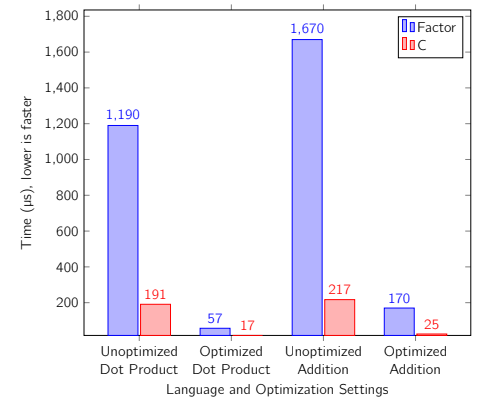
\includegraphics{factor_vs_c.png}
\caption{Factor vs.~C}
\end{figure}

In order to use Factor's foreign function interface (FFI), the C code
must be compiled into a library file and included with the Factor code.
However, different operating systems require different library file
formats, so such an implementation would require users to compile C code
themselves. Because Factor runs in a virtual machine, neither
programmers nor users have to deal with compiling the code to a specific
operating system---it's done automatically. If we implemented our
vocabulary in C, it would require a lot of additional work for our
vocabulary to be as accessible as the rest of the Factor source code.
Additionally, implementing our vocabulary in Factor also allows us to
use more high-level language features, such as automatic garbage
collection and higher-order functions like \texttt{map} and
\texttt{reduce}. We decided that the small performance improvement
provided by using C would not be worth the loss of portability or ease
of use.

\hypertarget{optimizing-native-factor}{%
\subsubsection{Optimizing Native
Factor}\label{optimizing-native-factor}}

The underlying implementation of the \texttt{tensor} class consists of
an \texttt{array} that holds the shape, and a \texttt{float-array} that
holds the values. Using a typed array increases speed as it avoids type
checking at runtime. Additionally, many of the words use strongly-typed
word definitions. This alone allowed for a huge speedup over dynamically
typed arrays.

To further optimize, we used SIMD operations, which allowed us to
perform vectorized computations. This was used to improve the
performance of element-wise arithmetic operations such as \texttt{t+},
sequence operations such as \texttt{sum}, and matrix multiplication.

To read more about how the vocabulary performed, including how it
compared to NumPy and the existing \texttt{math.matrices} vocabulary,
see the evaluation section.

\hypertarget{interface}{%
\subsubsection{Interface}\label{interface}}

One of our main goals was ease of use. To do this, we tried to make a
flexible and simple interface. We used multi-method dispatch when
implementing element-wise operations so that they can take either two
\texttt{tensor}s, or a number and a \texttt{tensor} in either order.

For example, the following code snippets all produce an output of
\texttt{t\{\ 5\ 6\ 7\ \}}:
\begin{itemize}
\item \texttt{t\{\ 0\ 1\ 2\ \}\ 5\ t+}
\item \texttt{5\ t\{\ 0\ 1\ 2\ \}\ t+}
\item \texttt{t\{\ 0\ 1\ 2\ \}\ t\{\ 5\ 5\ 5\ \}\ t+}
\end{itemize}

We also implemented the basic words necessary to apply sequence
operations and pretty printing.

\texttt{tensor}s can be turned to and from nested arrays using a parsing
word. Initialization of a one-dimensional \texttt{tensor} using the
parsing word \texttt{t\{} was shown above. A two-dimensional
\texttt{tensor} can be initialized as follows:
\texttt{t\{\ \{\ 0\ 1\ \}\ \{\ 2\ 3\ \}\ \}}.

The features implemented during this project cover only a small fraction
of the features provided by a library like NumPy.

\hypertarget{evaluation}{%
\subsection{Evaluation}\label{evaluation}}

In addition to operations over \texttt{tensor}s being correct, it was
important that they were fast---fast enough that they were useful in
situations requiring large matrices. Quantifying this more specifically,
our goal was to have all operations run within an order of magnitude of
NumPy, which is the gold standard for numerical programming libraries.
We also compared the performance of our vocabulary to the
\texttt{math.matrices} vocabulary in order to understand what
improvements we were actually providing the language.

\hypertarget{individual-operations}{%
\subsubsection{Individual Operations}\label{individual-operations}}

First, we benchmarked three individual operations: element-wise
addition, matrix multiplication, and transposition. The performance of
the \texttt{tensors} vocabulary came within an order of magnitude of
NumPy with some operations, but struggled with others. 

\begin{figure}
\centering
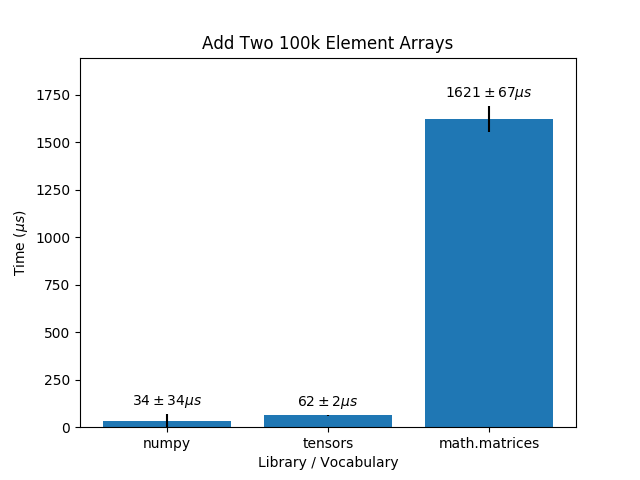
\includegraphics{add.png}
\caption{Add Two 100k Element Arrays}
\end{figure}

\begin{figure}
\centering
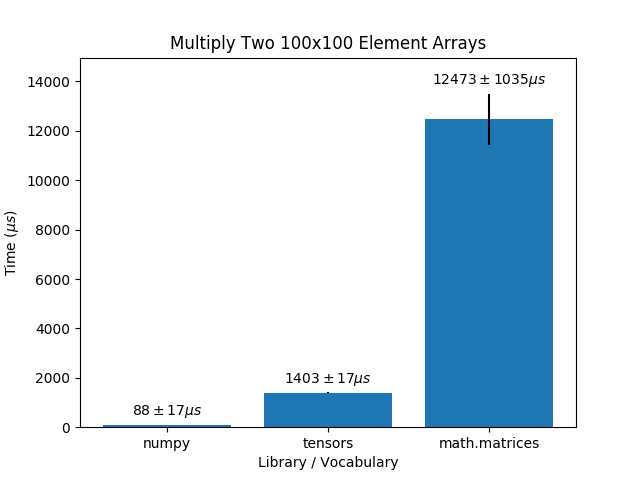
\includegraphics{matmul.png}
\caption{Multiply Two 100x100 Element Arrays}
\end{figure}

\begin{figure}
\centering
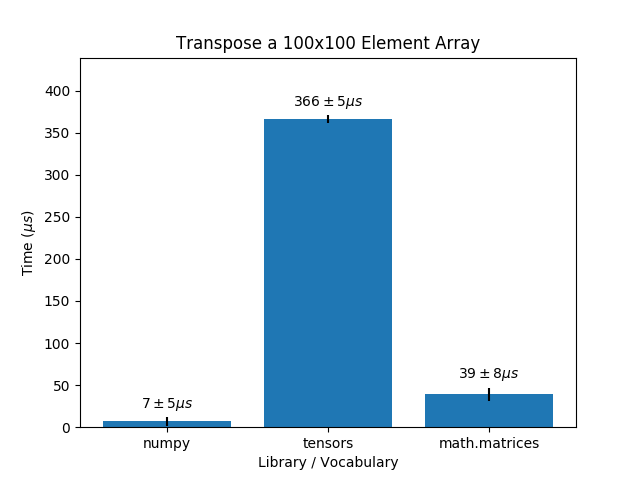
\includegraphics{transpose.png}
\caption{Transpose a 100x100 Element Array}
\end{figure}

Transpose in particular is much slower than both NumPy and
\texttt{math.matrices}. NumPy has constant-time transposition, so we did
not expect to always be within an order of magnitude of its speed.
However, we did want our transposition to be faster than
\texttt{math.matrices}. We believe that the speed of
\texttt{math.matrices} is due to the fact that the underlying
implementation consists of nested arrays rather than a single array, and
is therefore easier to map over. Furthermore, \texttt{tensor}
transposition must be generalizable to any dimension. Still, the current
performance is not ideal, and improving the speed of our transposition
is an important next step.

\hypertarget{proof-of-concept-linear-regression}{%
\subsubsection{Proof of Concept: Linear
Regression}\label{proof-of-concept-linear-regression}}

Additionally, as a proof of concept for our vocabulary, we combined a
series of operations to perform linear regression on the
\href{https://www.cs.toronto.edu/~delve/data/boston/bostonDetail.html}{Boston
housing dataset}. The implementation can be found
\href{https://github.com/factor/factor/blob/master/extra/tensors/demos/demos.factor}{here}.

Linear regression was the perfect proof of concept since it used all of
the features that we had implemented, including element-wise arithmetic
operations, matrix multiplication, and transposition. For only one
step---normalizing the features individually---did we need to deviate
from the provided functionality.

\begin{figure}
\centering
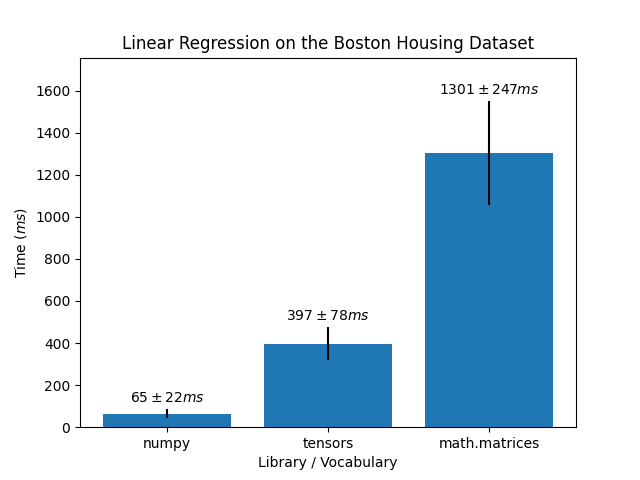
\includegraphics{linear_regression.png}
\caption{Linear Regression on the Boston Housing Dataset}
\end{figure}

As we see in the graph above, even on this larger integration test, the
\texttt{tensors} vocabulary performed within an order of magnitude of
NumPy on the given dataset, meeting our goal for the project. That being
said, it is still more than six times slower, and there is definitely
more work to be done in this area. 

\hypertarget{future-work-2}{%
\subsection{Future Work}\label{future-work-2}}

Broadly speaking, future work for this vocabulary can be broken up into
two major areas: improving \texttt{tensor}s' performance and usability.

There is still room for optimization with the currently implemented
words. Many of the implemented words are both more than an order of
magnitude slower than NumPy and do not scale as efficiently, most
notably \texttt{transpose}. This is an ongoing process, as each word can
ideally always get faster. One potential direction
to explore in looking for improvements to the performance of
\texttt{tensor} words is to compare the underlying assembly instructions
emitted by a C compiler such as GCC with the assembly instructions
emitted based on the Factor code for \texttt{tensors}. Understanding
where the differences are might give insight into how additional
instructions can be eliminated.

In addition, the performance of a number of \texttt{sequence} words can
be improved by providing \texttt{tensor}-specific implementations that
take advantage of the underlying structure of the \texttt{tensor}. This
includes many of the higher-order functions such as \texttt{map},
\texttt{2map}, and \texttt{reduce}. Finally, the \texttt{tensors}
vocabulary currently only supports 32-bit floats, and allowing
\texttt{tensor}s to store different types of numbers, including integers
and floats of different sizes would allow for additional performance
gains where floating point arithmetic is either not necessary or not
necessary at that precision. This would involve changing the underlying
implementation of \texttt{tensor}s and modifying multiple words.

To improve the usability of the \texttt{tensors} vocabulary, there are a
number of crucial features implemented with NumPy arrays that the
\texttt{tensors} vocabulary does not provide. These include
\href{https://docs.scipy.org/doc/numpy/user/basics.broadcasting.html}{broadcasting},
performing operations over specific axes (see the \emph{axes} variable
\href{https://numpy.org/doc/stable/reference/generated/numpy.transpose.html}{here}),
\href{https://numpy.org/doc/stable/reference/arrays.indexing.html}{index
slicing}, and more complicated mathematical operations. The versatility
that these operations provide would make using \texttt{tensor}s much
easier and more frictionless. These would be fairly intensive to
implement, and would involve modifying current operations as well as
adding new words.

Finally, the current vocabulary does not always do a good job of hiding
the underlying implementation from the user. Specifically, this becomes
a problem when trying to understand error messages. The addition of
better error checking---both more specific errors and checking for
errors earlier within operations---would make the vocabulary more
intuitive and easier to use. An example of this is with the parsing word
\texttt{t\{}, which could have tensor-specific errors for invalid
inputs. This would not be hard to implement, and would consist of adding
extra cases to the \texttt{\textgreater{}tensor} word.

\end{document}
